\subsection{The Heart-on-a-Chip platform}
\label{HoC}

\begin{figure}[!t]
	\centering
	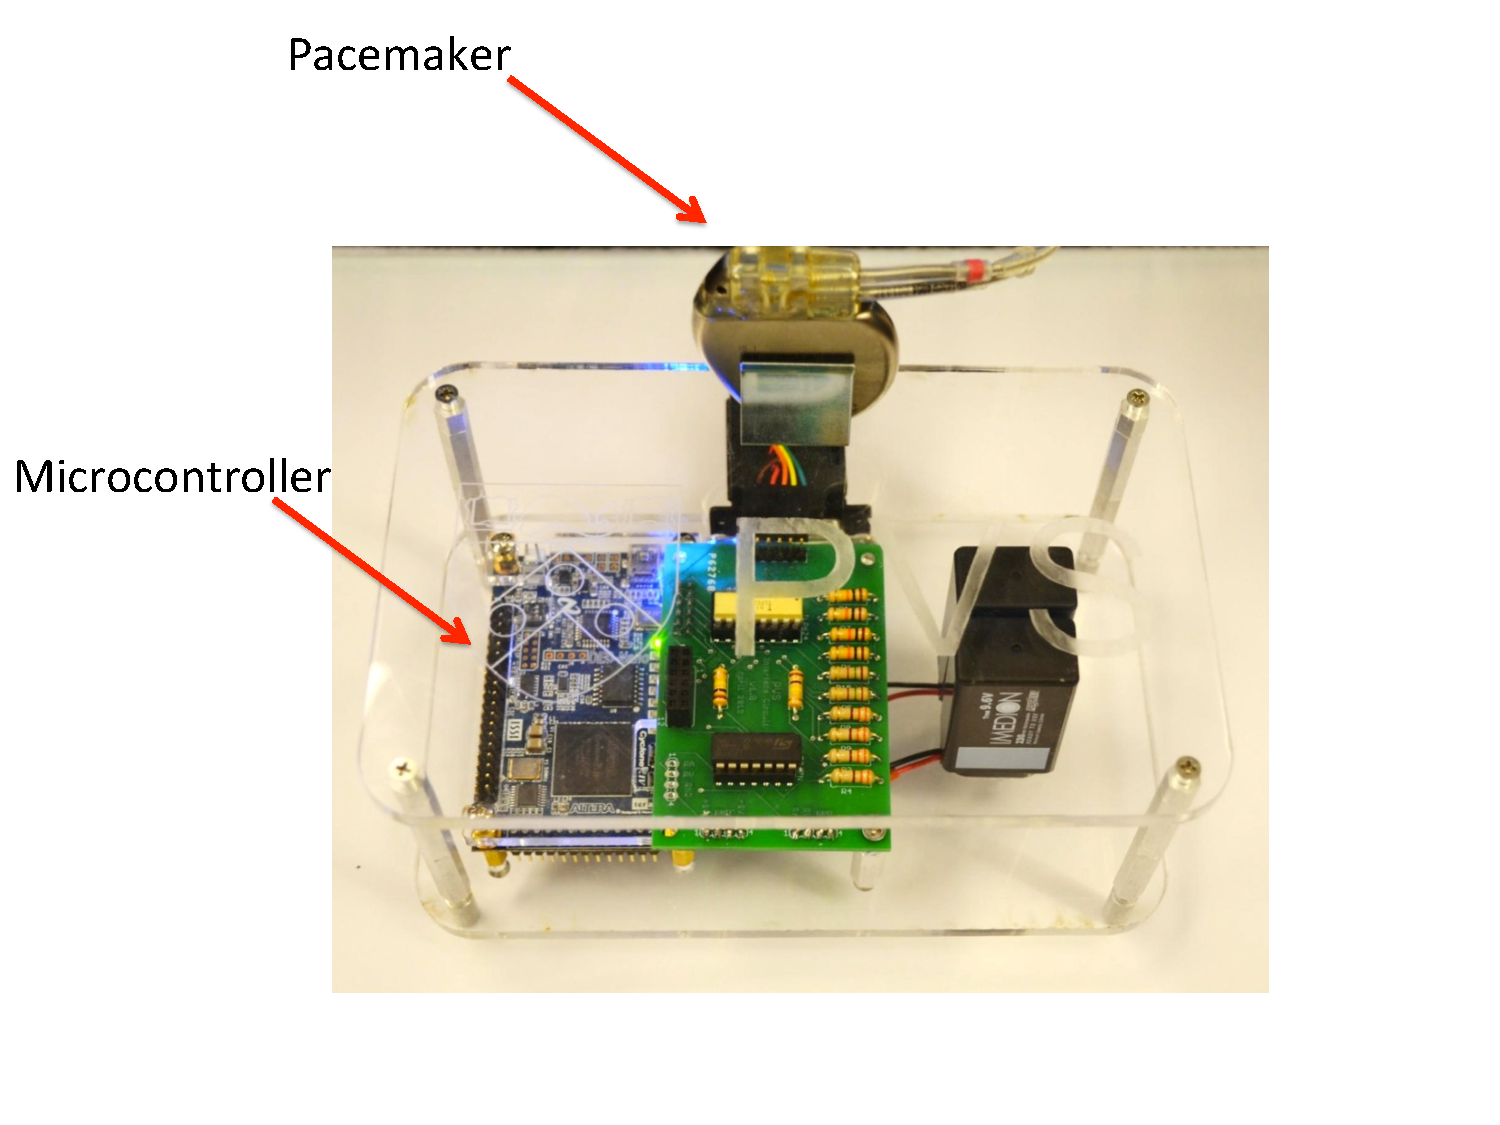
\includegraphics[scale=0.4]{HOCannotated.pdf}		
	\caption{\small Heart-on-a-Chip platform, showing the pacemaker, the microcontroller running the VHM code, and the monitors.}
	\label{fig:hoc}
\end{figure} 
Our closed-loop testing scheme ranges across different stages of the development process. Closed-loop testing can not only be performed on pacemaker models and code, but also on off-the-shelf pacemakers. \figref{hoc} shows the Heart-on-a-Chip (HoC) platform for closed-loop testing of pacemakers. The platform consists of a micro-controller with heart model implemented on it, and an analog interface which convert heart signals
%Before describing the advantages of closed-loop testing, we introduce the Heart-on-a-Chip (HoC) platform, which will be used for the development of closed-loop testers.
%See Fig.~\ref{fig:hoc}.
%\todo[inline]{more...}
